\subsection{Recopilaci\'on de datos del software y desempe\~no 2}
    Los datos que han sido recopilados hasta el momento con los
        que est\'an en base a las pruebas con los mapas que
        representan ya un escenario de la vida real. En la simulaci\'on
        hay distintos estados que se pueden colocar en el lienzo del
        estado inicial antes de disparar el simulador para obtener la
        ruta. Uno de estos estados es el estado 2, el cual representa
        un repelente que, a efectos pr\'acticos de nuestro software, son
        la representaci\'on de lo que fueran paredes u obst\'aculos en el
        entorno o el mapa que se coloca como estado inicial.
    \vskip 0.5cm
    %figura
    \begin{figure}[htbp]
        \centering
        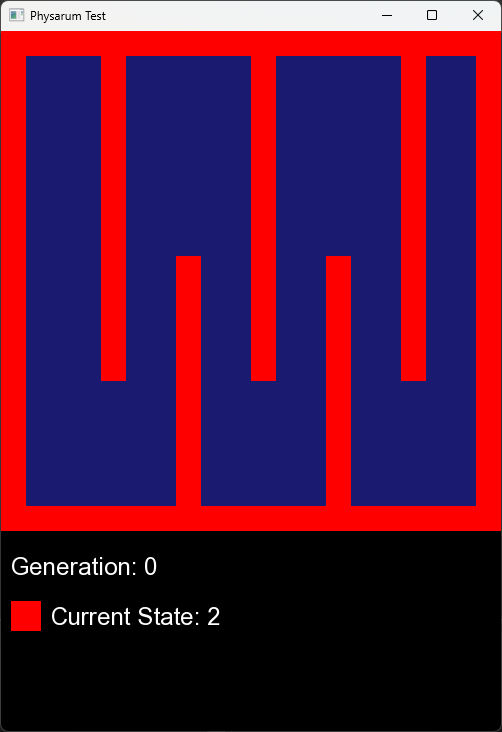
\includegraphics[width=0.5\textwidth]{./images/Pruebas/simulador/image059.png}
        \caption{Una configuraci\'on inicial con osbtaculos}
        \label{fig:Ruta 59}
    \end{figure}
    \vskip 0.5cm
    El repelente tiene como funci\'on en el simulador, impedir el
        paso del Physarum en los puntos donde este se encuentre,
        por lo que funciona bien como si fuera la representaci\'on de
        paredes o barreras de los mapas en donde no se puede
        avanzar en la vida real.
        \vskip 0.5cm
    As\'i que esta vez, las pruebas para medir el desempe\~no, que
        como anteriormente se mencion\'o, se hacen midiendo el
        tiempo entre el avance de un estado y el siguiente, fueron
        sobre un estado inicial donde se coloca inicialmente una
        serie de obst\'aculos para llegar al destino final, esto es como
        si fuera un laberinto por el cual el Physarum debe de pasar
        para poder llegar a su destino. Esto hace que la evaluaci\'on
        en general tarde un poco m\'as que si fuera un mapa o estado
        inicial sin alg\'un tipo de obst\'aculo.
    \vskip 0.5cm
    A continuaci\'on, se muestran algunos de los resultados
        obtenidos con algunas configuraciones.
    \vskip 0.5cm
    %figura
    \begin{figure}[htbp]
        \centering
        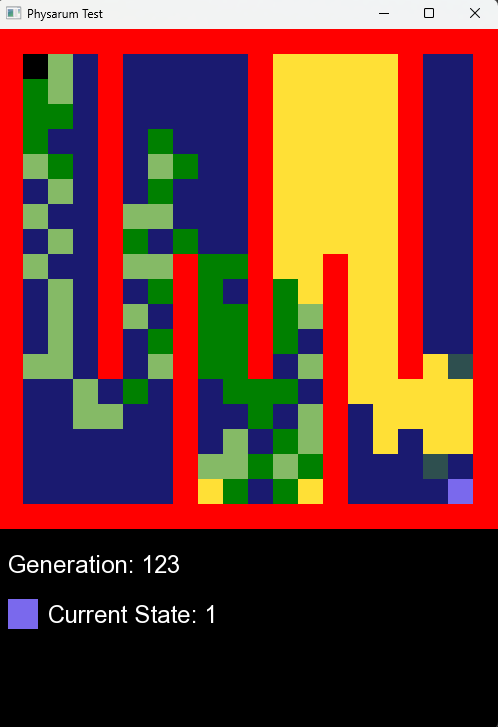
\includegraphics[width=0.5\textwidth]{./images/Pruebas/simulador/image061.png}
        \caption{Expansi\'on del algoritmo de Physarum.}
        \label{fig:Ruta 61}
    \end{figure}
    \vskip 0.5cm
    %figura
    \begin{figure}[htbp]
        \centering
        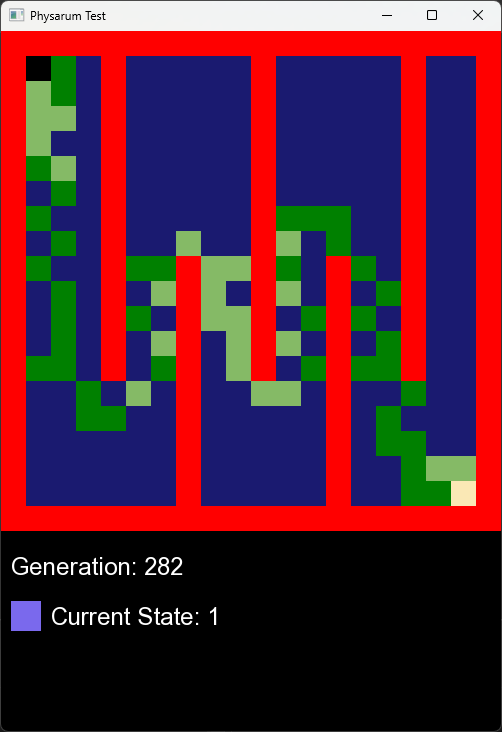
\includegraphics[width=0.5\textwidth]{./images/Pruebas/simulador/image063.png}
        \caption{Ruta generada a partir de una configuraci\'on inicial complicada.}
        \label{fig:Ruta 63}
    \end{figure}
    \vskip 0.5cm
    %figura
    \begin{figure}[htbp]
        \centering
        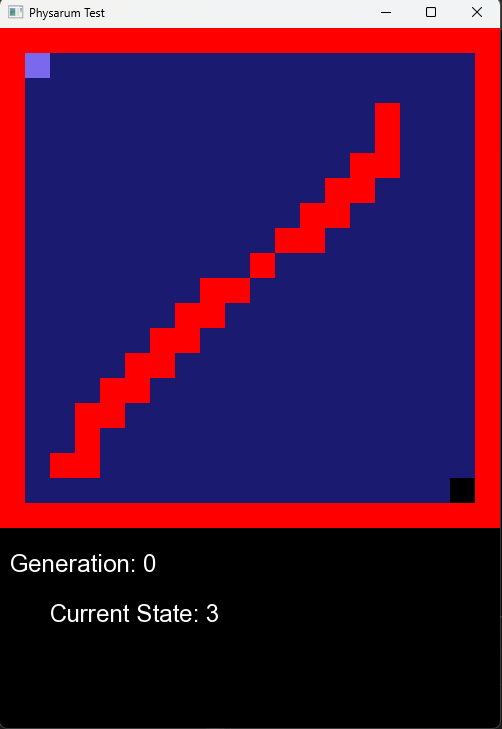
\includegraphics[width=0.5\textwidth]{./images/Pruebas/simulador/image065.png}
        \caption{Estado inicial de una configuraci\'on.}
        \label{fig:Ruta 65}
    \end{figure}
    \vskip 0.5cm
    %figura
    \begin{figure}[htbp]
        \centering
        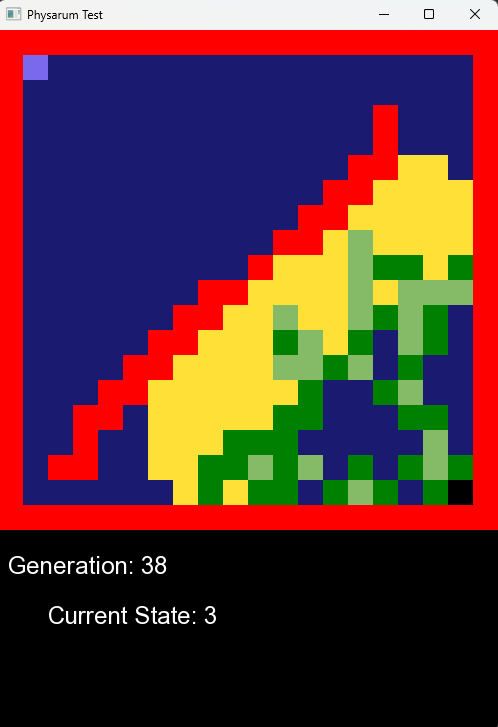
\includegraphics[width=0.5\textwidth]{./images/Pruebas/simulador/image067.png}
        \caption{Expansi\'on del algoritmo del Physarum con una pared diagonal en medio.}
        \label{fig:Ruta 67}
    \end{figure}
    \vskip 0.5cm
    %figura
    \begin{figure}[htbp]
        \centering
        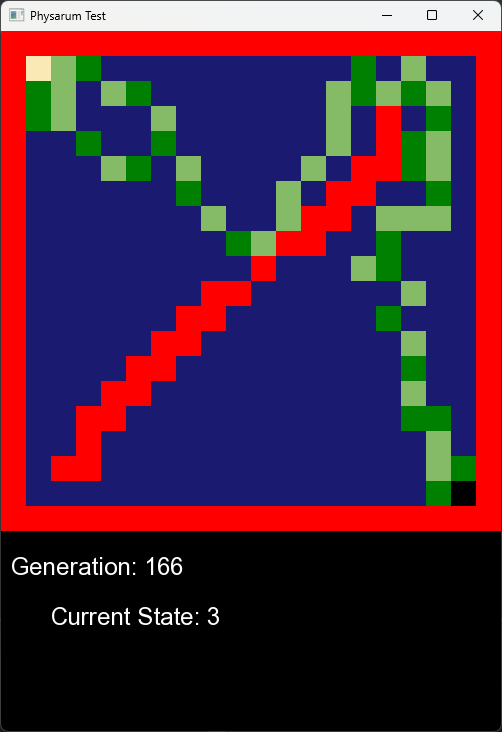
\includegraphics[width=0.5\textwidth]{./images/Pruebas/simulador/image069.png}
        \caption{Generaci\'on de la ruta satisfactoria que es generada durante la ejecuci\'on y finalizaci\'on del algoritmo.}
        \label{fig:Ruta 69}
    \end{figure}
    \vskip 0.5cm
    %figura
    \begin{figure}[htbp]
        \centering
        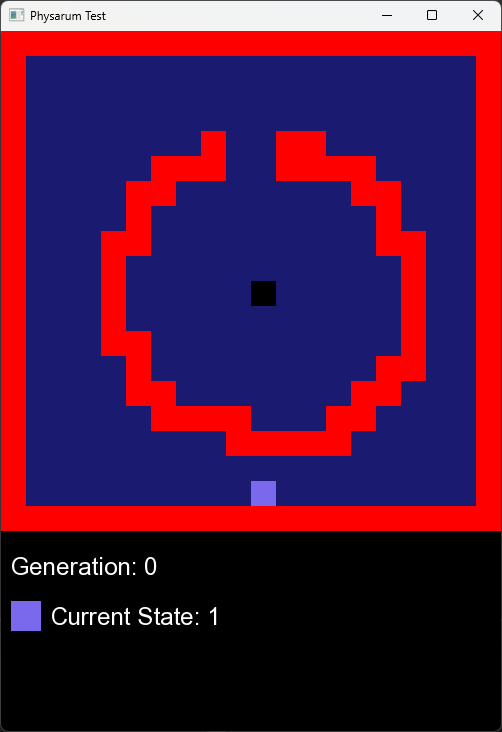
\includegraphics[width=0.5\textwidth]{./images/Pruebas/simulador/image071.png}
        \caption{Estado inicial con configuraci\'on circular.}
        \label{fig:Ruta 71}
    \end{figure}
    %figura
    \begin{figure}[htbp]
        \centering
        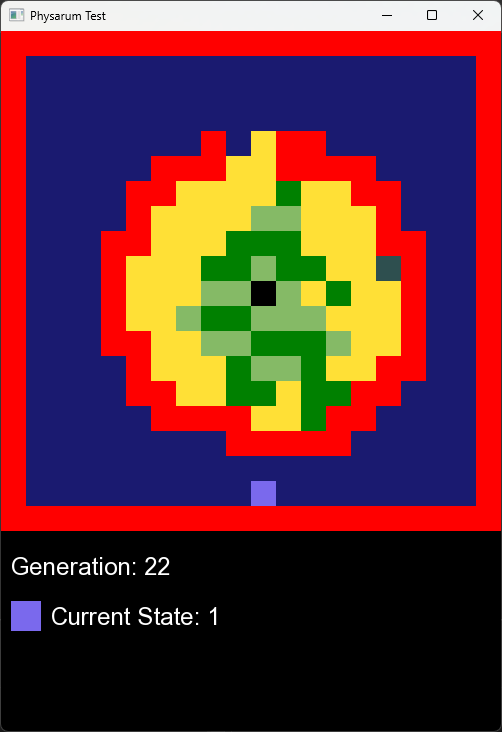
\includegraphics[width=0.5\textwidth]{./images/Pruebas/simulador/image073.png}
        \caption{Expansi\'on con una configuraci\'on de repelentes circular.}
        \label{fig:Ruta 73}
    \end{figure}
    \vskip 0.5cm
    %figura
    \begin{figure}[htbp]
        \centering
        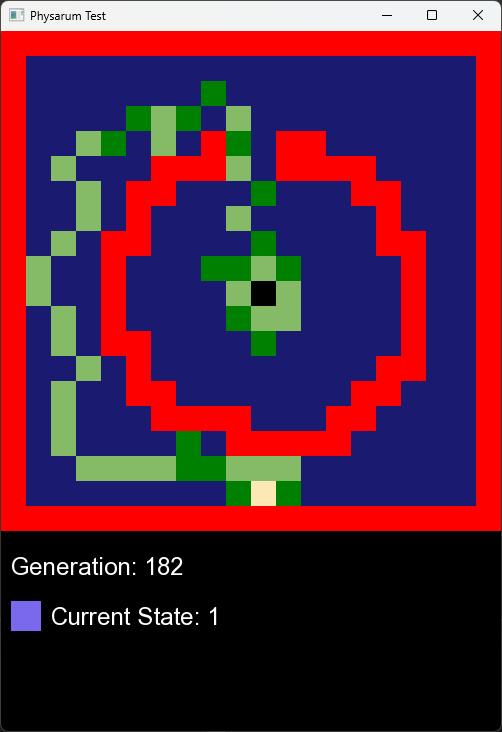
\includegraphics[width=0.5\textwidth]{./images/Pruebas/simulador/image075.png}
        \caption{Ruta generada despu\'es de la finalizaci\'on de la simulaci\'on.}
        \label{fig:Ruta 75}
    \end{figure}
    \clearpage